\documentclass[12pt]{article}

% Packages
\usepackage[margin=1in]{geometry}
\usepackage{setspace}
\usepackage{amsmath}
\usepackage{amssymb}
\usepackage{graphicx}
\usepackage{xcolor}
\usepackage{booktabs}
\usepackage{array}
\usepackage{tabularx}
\usepackage{hyperref}

% Title information
\title{Optimal Flood Policy}
\author{Taco Prins, Lennard Schlattmann, and Daniel Jonas Schmidt}
\date{\today}

\begin{document}

\maketitle

\section{Motivation}
\begin{itemize}
    \item Households have heterogeneous flood risk beliefs. Those who underestimate flood risk may not buy insurance or invest enough in private adaptation measures. A universal flood insurance mandate, which would ensure that even those who underestimate flood risk are insured, is often legally and politically infeasible.
    \item This creates a potential role for government intervention in the form of flood insurance subsidies, subsidies for private adaptation measures, disaster relief programs, or a combination of all policies.
    \item Subsidies can increase insurance and adaptation towards their socially optimal level, but with sufficient heterogeneity in beliefs, there will always be a group of households that underestimate flood risk enough to stay uninsured and under-adapted even with subsidies in place. 
    \item Disaster relief programs provide a safety net for uninsured households, but they also reduce incentives to buy flood insurance or invest in private adaptation measures. 
    \item What is the socially optimal mix of these policies in the presence of heterogeneous flood risk beliefs? Is it optimal to use all available policy instruments, or only a subset? How close is the current US policy to the optimum?
\end{itemize}

\section{Baseline model}

Consider a one-period model with one region. The government has a fixed budget $B$ dedicated to flood policies and can choose between two instruments: an insurance subsidy $s$ and a disaster relief fraction $a$.

\subsection{Household Problem}

Each household has wealth $w$ and faces a flood that occurs with true probability $p$ and causes damage $d$. Households differ in their subjective flood probability $q$, distributed across the population according to the CDF $F(q)$. There is no misperception about damage conditional on flood occurrence.

\begin{itemize}
    \item The government subsidizes flood insurance relative to the actuarially fair price, so an insured household pays $(1-s)pd$.
    \item The government provides disaster relief covering a fraction $a$ of damage for uninsured households that experience a flood.
\end{itemize}

\subsubsection*{Value Functions}
\begin{itemize}
    \item Insured: $V_I(s) = u(c_I) = u(w - (1-s)pd)$
    \item Uninsured (true): $V_U(a) = (1-q)\,u(c_{U,N}) + q\,u(c_{U,F}) = (1-q) u(w) + q u(w - (1-a)d)$
    \item Uninsured (perceived): $\tilde{V}_U(q,a) = (1-p)\,u(c_{U,N}) + p\,u(c_{U,F})$
\end{itemize}

\subsubsection*{Optimal Behavior}
A household buys insurance if $V_I(s) > \tilde{V}_U(q,a)$. Setting $V_I(s) = \tilde{V}_U(q^*,a)$ and solving for the threshold belief yields
\begin{equation}
    q^*(s,a) = \frac{u(c_{U,N}) - u(c_I)}{u(c_{U,N}) - u(c_{U,F})} \label{eq:qstar}
\end{equation}
Households with $q > q^*(s,a)$ buy insurance; those with $q \leq q^*(s,a)$ do not.

\subsection{Government Problem}

The government maximizes social welfare subject to its budget constraint. The social planner evaluates household welfare using the true flood probability $p$. Denoting the insurance take-up rate by $I(s,a) = 1 - F(q^*(s,a))$, the government's problem is
\begin{equation}
    S(s,a) = V_I(s)\cdot I(s,a) + V_U(a)\cdot\bigl(1-I(s,a)\bigr) \label{eq:welfare}
\end{equation}
subject to
\begin{equation}
    B = pd\bigl[s\,I(s,a) + a\,\bigl(1-I(s,a)\bigr)\bigr]. \label{eq:budget}
\end{equation}
The Lagrangian is
\[
    \mathcal{L}(s,a,\lambda) = S(s,a) + \lambda\!\left[B - pd\bigl(s\,I(s,a) + a\,\bigl(1-I(s,a)\bigr)\bigr)\right],
\]
where $\lambda$ is the shadow value of the budget constraint.

\subsubsection*{First-Order Conditions}

\begin{align}
    \frac{\partial\mathcal{L}}{\partial s} &=
        (V_I-V_U)\,\frac{\partial I}{\partial s}
        + \frac{\partial V_I}{\partial s}\cdot I
        - \lambda\,pd\!\left[
            I + (s-a)\,\frac{\partial I}{\partial s}
        \right] = 0 \label{eq:foc_s} \\[12pt]
    \frac{\partial\mathcal{L}}{\partial a} &=
        (V_I-V_U)\,\frac{\partial I}{\partial a}
        + \frac{\partial V_U}{\partial a}\cdot(1-I)
        - \lambda\,pd\!\left[
            (1-I) + (s-a)\,\frac{\partial I}{\partial a}
        \right] = 0 \label{eq:foc_a}
\end{align}

\subsubsection*{Marginal Value of Public Funds}

Rearranging each first-order condition so that the welfare gain per dollar of fiscal cost equals $\lambda$ gives the marginal value of public funds (MVPF) for each instrument:

\begin{align}
    \text{MVPF}_s &= \frac{
        (V_I-V_U)\,\dfrac{\partial I}{\partial s}
        + \dfrac{\partial V_I}{\partial s}\cdot I
    }{
        pd\!\left[I + (s-a)\,\dfrac{\partial I}{\partial s}\right]
    } \label{eq:mvpf_s_vf} \\[14pt]
    \text{MVPF}_a &= \frac{
        (V_I-V_U)\,\dfrac{\partial I}{\partial a}
        + \dfrac{\partial V_U}{\partial a}\cdot(1-I)
    }{
        pd\!\left[(1-I) + (s-a)\,\dfrac{\partial I}{\partial a}\right]
    } \label{eq:mvpf_a_vf}
\end{align}

\noindent The numerators capture the marginal welfare gain from increasing the instrument:
\begin{itemize}
    \item \textbf{Internality correction.} Households at the margin $q = q^*$ misperceive their flood risk. Switching them into (or out of) insurance changes social welfare by $(V_I - V_U)$ per switcher, and each instrument shifts $\partial I/\partial s$ (or $\partial I/\partial a$) households across the margin. Because $V_I(s) = \tilde{V}_U(q^*,a)$ at the threshold by definition of $q^*$, the welfare gap reflects the difference between applying the true versus subjective probability to the uninsured outcome:
    \begin{equation}
        V_I - V_U = \tilde{V}_U(q^*,a) - V_U(a) = (p-q^*)\,\Delta u, \label{eq:internality}
    \end{equation}
    where $\Delta u \equiv u(c_{U,N}) - u(c_{U,F}) > 0$ is the utility gain from avoiding flood damage. Following Allcott, Lockwood, and Taubinsky (2019), we call this the \emph{internality correction}. It is positive when $q^* < p$ (the marginal household underestimates flood risk), so the subsidy corrects an internality by switching underinsured households to coverage. For disaster relief, $\partial I/\partial a < 0$, so the same term is negative: relief crowds marginal households out of insurance.
    \item \textbf{Direct benefit to recipients.} Each instrument directly benefits its existing recipients. The subsidy reduces premiums for all $I$ insured households by $\partial V_I/\partial s = pd\,u'(c_I)$ per unit. Disaster relief improves outcomes for all $1-I$ uninsured households that experience a flood by $\partial V_U/\partial a = pd\,u'(c_{U,F})$ per unit. Because uninsured flood victims are poorer ($c_{U,F} < c_I$), their marginal utility is higher: a dollar of relief generates more direct utility than a dollar of subsidy.
\end{itemize}
The denominators capture the marginal fiscal cost of increasing the instrument:
\begin{itemize}
    \item \textbf{Direct cost.} Each instrument has a direct cost of $pd$ per recipient: the subsidy costs $pd$ for each of the $I$ insured households, while relief costs $apd$ for each of the $(1-I)$ uninsured households that experience a flood.
    \item \textbf{Fiscal externality.} Each instrument has a fiscal externality from households switching between instruments: a switcher moves from costing $apd$ in relief to $spd$ in subsidy (or vice versa), changing government expenditure by $(s-a)pd$ per switcher.
\end{itemize}

\paragraph{Take-up responses.} Since insurance coverage $I = 1 - F(q^*)$ depends on the threshold belief $q^*$, the take-up responses $\partial I/\partial s$ and $\partial I/\partial a$ depend on how $q^*$ changes with each instrument:
\begin{align}
    \frac{\partial I}{\partial s} &= -f(q^*)\,\frac{\partial q^*}{\partial s}
    = \frac{f(q^*)\,pd\,u'(c_I)}{\Delta u}, \label{eq:dI_s} \\
    \frac{\partial I}{\partial a} &= -f(q^*)\,\frac{\partial q^*}{\partial a}
    = -\frac{f(q^*)\,q^*d\,u'(c_{U,F})}{\Delta u}. \label{eq:dI_a}
\end{align}

\paragraph{MVPF in terms of deep parameters.}
Substituting the take-up responses together with $V_I-V_U=(p-q^*)\Delta u$, $\partial V_I/\partial s = pd\,u'(c_I)$, and $\partial V_U/\partial a = pd\,u'(c_{U,F})$ into equations~\eqref{eq:mvpf_s_vf}--\eqref{eq:mvpf_a_vf} yields
\begin{align}
    \text{MVPF}_s &= \frac{u'(c_I)\bigl[I + (p-q^*)\,f(q^*)\bigr]}{I + (s-a)\,\dfrac{pd\,u'(c_I)\,f(q^*)}{\Delta u}}, \label{eq:mvpf_s} \\[14pt]
    \text{MVPF}_a &= \frac{u'(c_{U,F})\!\left[(1-I) - \dfrac{(p-q^*)q^*f(q^*)}{p}\right]}{(1-I) - (s-a)\,\dfrac{q^*d\,u'(c_{U,F})\,f(q^*)}{\Delta u}}. \label{eq:mvpf_a}
\end{align}

Each numerator decomposes into a direct benefit to inframarginal recipients and a pigouvian correction from the behavioral response at the margin; each denominator decomposes into a direct fiscal cost and a fiscal externality from switching.

\begin{itemize}
    \item \textbf{Direct benefit.} The leading factor $u'(c_I)$ in $\mathrm{MVPF}_s$ and $u'(c_{U,F})$ in $\mathrm{MVPF}_a$ is the marginal utility of the primary recipient group. Multiplied by $I$ (or $1-I$) and by $pd$, it gives the direct welfare gain per unit of government spending: a dollar of premium relief is worth $u'(c_I)$ to each insured household, and a dollar of disaster relief is worth $u'(c_{U,F})$ to each uninsured flood victim. Because $c_{U,F} < c_I$, we have $u'(c_{U,F}) > u'(c_I)$, which is the fundamental reason disaster relief tends to have a higher MVPF.

    \item \textbf{Pigouvian correction in $\mathrm{MVPF}_s$.} The pigouvian term $(p-q^*)\cdot u'(c_I)\cdot f(q^*)$ measures the \emph{aggregate misperception at the policy margin}: the density $f(q^*)$ of households that a marginal subsidy nudges into coverage, each carrying a belief gap $(p-q^*)$ — the fraction of true flood risk they are ignoring. The product $(p-q^*)f(q^*)$ is large when marginal households are both numerous and badly miscalibrated. The utility scale $\Delta u$ does not appear, because it governs both how valuable each switch is (the internality $(p-q^*)\Delta u$ grows with $\Delta u$) and how hard switching is to induce (the threshold $q^*$ moves by $1/\Delta u$ per unit subsidy, since $q^*$ is a ratio normalised by $\Delta u$). These two effects cancel exactly, leaving the pigouvian correction independent of the utility scale.

    \item \textbf{Pigouvian correction in $\mathrm{MVPF}_a$.} The crowd-out pigouvian loss is $(p-q^*)\cdot\frac{q^*}{p}\cdot u'(c_{U,F})\cdot f(q^*)$ — the same aggregate misperception $(p-q^*)f(q^*)$, scaled down by $q^*/p$. This factor arises because the crowd-out rate is governed by the marginal household's \emph{subjective} flood probability $q^*$: a household drops insurance only to the extent it perceives flood risk, so the crowd-out response is proportional to $q^*d$ rather than $pd$. Dividing by the actuarial rate $p$ (at which the direct relief benefit is priced) yields $q^*/p < 1$. Since marginal households underestimate flood risk ($q^* < p$), the crowd-out pigouvian loss is always smaller than the corresponding internality gain in $\mathrm{MVPF}_s$.

    \item \textbf{Fiscal externalities.} Each denominator is the direct per-unit fiscal cost ($I$ for the subsidy, $1-I$ for relief) adjusted for households switching between instruments. A household switching from uninsured to insured moves from costing $apd$ in expected relief to $spd$ in subsidy, a net fiscal change of $(s-a)pd$ per switcher. When $s > a$, this raises the denominator of $\mathrm{MVPF}_s$ (crowd-in is costly) and lowers the denominator of $\mathrm{MVPF}_a$ (crowd-out saves money), pushing the two MVPFs further apart.

    \item \textbf{Limiting case.} When beliefs are correct ($q^* = p$) or the density at the margin is negligible ($f(q^*) \approx 0$), all pigouvian and fiscal externality terms vanish. The formulas collapse to $\mathrm{MVPF}_s = u'(c_I)$ and $\mathrm{MVPF}_a = u'(c_{U,F})$: marginal values equal the marginal utilities of the respective recipients, as in a standard social insurance formula.
\end{itemize}

At an interior optimum, $\text{MVPF}_s = \text{MVPF}_a$: neither instrument can be improved at the margin. Away from the optimum, the marginal dollar should go to the instrument with the higher MVPF.

\section{Extensions}
\begin{itemize}
    \item Administration costs for flood insurance and disaster relief
    \item Private adaptation measures
    \item What is the optimal budget dedicated to flood policies? Compare marginal value of public funds with marginal cost of public funds
    \item Correlation of flood risk beliefs with income and/or wealth
    \item Heterogeneity in risk aversion
    \item Public adaptation measures
    \item Liquidity-provision policies (disaster loans, 401k withdrawals, mortgage relief)
    \item Households migrate into flood-prone areas because of government support (sorting based on beliefs)
    \item Continuous flood insurance decision
    \item Continuous flood damage
\end{itemize}

\subsection{Continuous flood damage}

\paragraph{Flood damage distribution.}
Flood occurs with true probability $p$. Conditional on flood, damage is random:
$\textcolor{red}{D\sim G}$ with mean $\textcolor{red}{\bar d\equiv\mathbb{E}[D]}$.
Households misperceive only flood probability: $q\sim F(q)$. 

\paragraph{Policies and consumption.}
Insurance is full coverage priced at actuarially fair expected loss, subsidized at rate $s$:
$c_I=w-(1-s)p\textcolor{red}{\bar d}$.
Uninsured consumption: $c_{U,N}=w$ (no flood), and
$c_{U,F}(\textcolor{red}{D})=w-(1-a)\textcolor{red}{D}$ (flood with relief fraction $a$). 

\paragraph{Threshold belief and take-up.}
The marginal (indifferent) belief is
\[
q^*(s,a)=
\frac{u(w)-u\!\left(w-(1-s)p\textcolor{red}{\bar d}\right)}
{u(w)-\textcolor{red}{\mathbb{E}[u(w-(1-a)D)]}}
=
\frac{u(w)-u(c_I)}{\textcolor{red}{\Delta u(a)}},
\]
and insurance take-up is $I(s,a)=1-F(q^*(s,a))$. 

\paragraph{Welfare and budget constraint.}
Planner welfare keeps the same form:
\[
S(s,a)=V_I(s)\,I(s,a)+V_U(a)\,[1-I(s,a)],
\]
with $V_I(s)=u(c_I)$ and
$V_U(a)=(1-p)u(w)+p\,\textcolor{red}{\mathbb{E}[u(w-(1-a)D)]}$.
The budget constraint is unchanged up to replacing $d$ by $\textcolor{red}{\bar d}$:
\[
B=p\textcolor{red}{\bar d}\Big[s\,I(s,a)+a\,(1-I(s,a))\Big].
\]

\paragraph{Internality correction.}
At the margin, $V_I(s)=\widetilde V_U(q^*,a)$, so
\[
V_I-V_U=(p-q^*)\,\textcolor{red}{\Delta u(a)},
\]
i.e., the welfare gain from switching the marginal household is still proportional
to the belief gap $(p-q^*)$ times the (now expected) utility loss from being uninsured
under flood risk. 

\paragraph{Direct marginal benefits.}
Subsidy marginal benefit remains
\[
\frac{\partial V_I}{\partial s}
= p\textcolor{red}{\bar d}\,u'(c_I).
\]
Relief now targets high-loss states via a damage-weighted marginal utility:
\[
\frac{\partial V_U}{\partial a}
= p\,\textcolor{red}{\mathbb{E}\!\left[D\,u'\!\left(w-(1-a)D\right)\right]},
\]
which exceeds $p\bar d\,u'(w-(1-a)\bar d)$ under concavity and heavy tails.

\paragraph{Summary.}
Relative to the baseline with deterministic damage, all changes enter through expectations over realized damage $D$, replacing point evaluations at $d$ by mean damage $\bar{d}$ in fiscal terms and by damage‑weighted marginal utilities in the welfare effects of disaster relief.

\textcolor{orange}{\paragraph{Comment lennard:}
One implication of this extension might be that the optimal relief fraction $a$ also depends on the shape of the damage distribution $G$. 
For example, if $G$ has a heavy right tail, then the marginal benefit of relief is higher because it provides more insurance against extreme losses. 
This could lead to a higher optimal relief fraction compared to the case with deterministic damage.}

\subsection{Risk aversion heterogeneity}

We now explicitly assume a CRRA utility function, i.e. $u(c)=\frac{c^{1-\gamma}}{1-\gamma}$. The marginal indifferent belief of an agent with CRRA $\gamma$ is 
\begin{equation}
    q^*(s,a;\gamma) = \frac{w^{1-\gamma} - (w-(1-s)pd)^{1-\gamma}}{w^{1-\gamma} - (w-(1-a)d)^{1-\gamma}}. \label{eq:qstargamma}
\end{equation}

Risk aversion $\gamma$ has a considerable affect on this threshold value. Figure \ref{fig:qstar_gamma} shows how $q^*$ varies with $\gamma$, using $s=13.9\%$ and $a=7.4\%$.
\begin{figure}[h!]
    \centering
    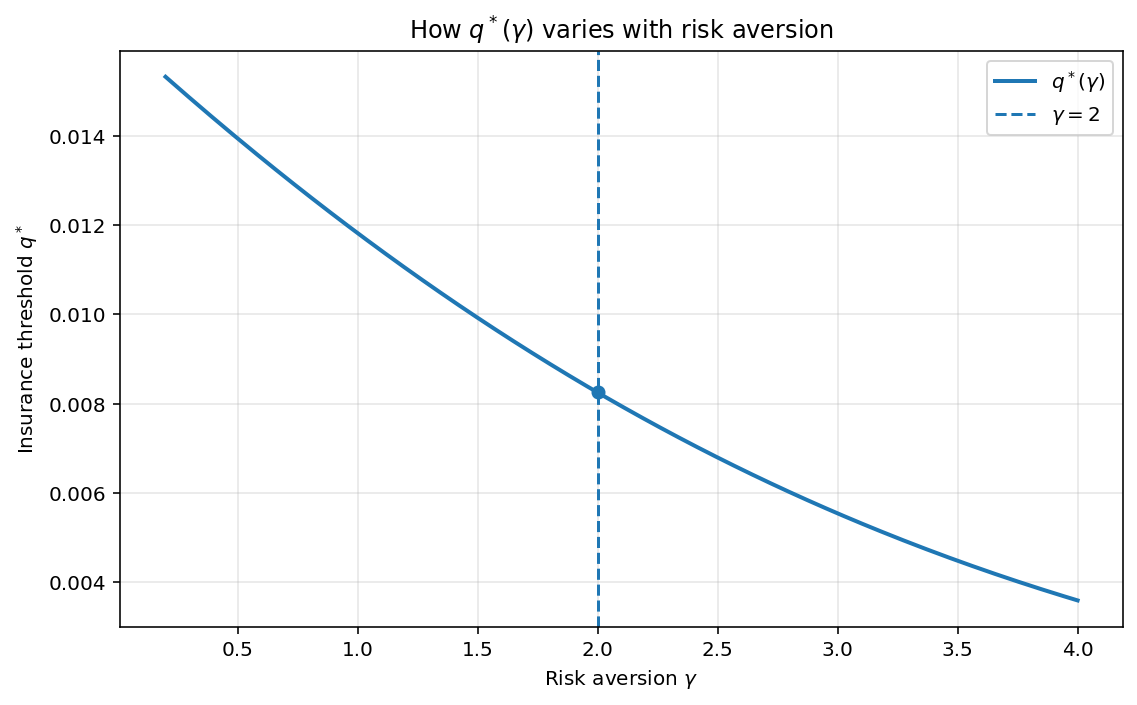
\includegraphics[width=0.7\linewidth]{figures/Dependence_q_gamma.png}
    \caption{Dependence of the insurance threshold $q^*$ on risk aversion $\gamma$, evaluated at $s=13.9\%$ and $a=7.4\%$.}
    \label{fig:qstar_gamma}
\end{figure}

However, dispersion in risk aversion does not seem to affect very much how the fraction of insured households responds to policy. Figure \ref{fig:fracinsuredgamma} below shows the fraction of insured households as a function of $a$, with $s$ adjusting to meet the government budget constraint. The left-hand panel shows this fraction with $\sigma=0.7\%$, and the right-hand panel with $\sigma=1.0\%$. CRRA $\gamma$ is assumed to follow a lognormal distribution with mean $2$. From this numerical evidence, dispersion in $\gamma$ thus does not alter by very much the fundamental trade-off between compensating flood-affected households and maximising insurance coverage.  
    
\begin{figure}[h]
\centering
\begin{minipage}{0.48\textwidth}
\centering
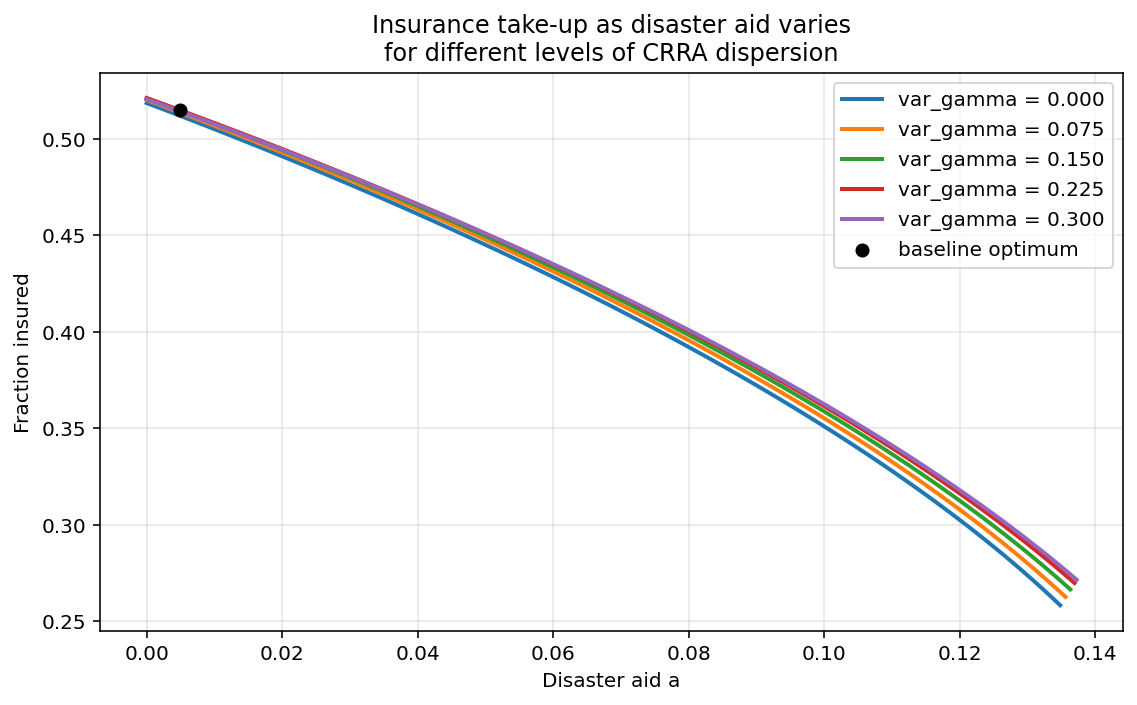
\includegraphics[width=\textwidth]{figures/Dependence_insuranceratio_vargamma.png}
\caption{Fraction of insured household as a function of policy $a,s$ and variance of CRRA $\gamma$, with $\sigma_q=0.7\%$}
\end{minipage}
\hfill
\begin{minipage}{0.48\textwidth}
\centering
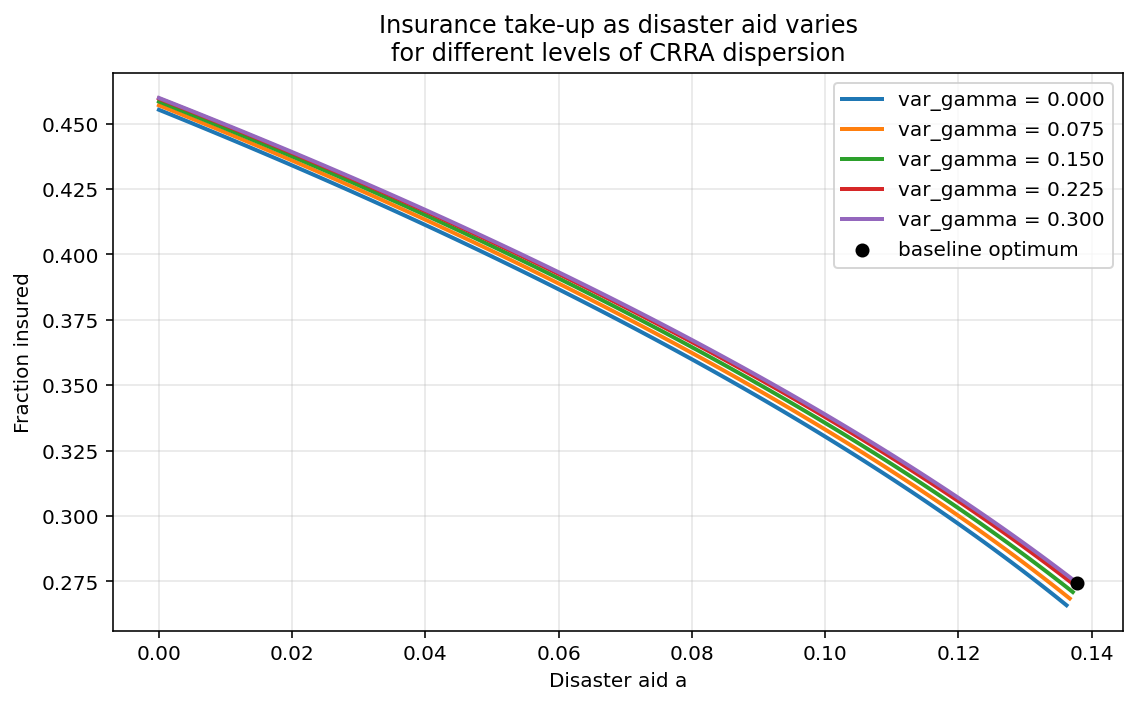
\includegraphics[width=\textwidth]{figures/Dependence_insuranceratio_vargamma_varq0.01.png}
\caption{Fraction of insured household as a function of policy $a,s$ and variance of CRRA $\gamma$, with $\sigma_q=1.0\%$}
\end{minipage}
\label{fig:fracinsuredgamma}
\end{figure}   

\subsubsection{Social planner problem with heterogeneous risk aversion}

We assume that risk aversion is heterogeneous across households, with
\[
\gamma \sim \text{LogNormal}(\mu_\gamma, \sigma_\gamma^2).
\]

When preferences are heterogeneous, utility is not directly comparable across individuals, as cardinal utility depends on the normalization of the utility function. To obtain a welfare measure that is comparable across households, we evaluate outcomes in terms of \emph{certainty-equivalent consumption}.

\paragraph{Certainty-equivalent consumption}

Fix a household with risk aversion $\gamma$. If the household purchases insurance, consumption is deterministic and given by
\[
c_I(s) = w - (1-s)\pi d.
\]
Hence, its certainty-equivalent consumption is simply
\[
c_I^{CE}(s;\gamma) = c_I(s).
\]

If instead the household remains uninsured, it faces flood risk. Expected utility is given by
\[
V_U(s,a;\gamma) = (1-p)u(w;\gamma) + p\,u\bigl(w-(1-a)d;\gamma\bigr),
\]
and the corresponding certainty-equivalent consumption $c_U^{CE}(s,a;\gamma)$ is implicitly defined by
\[
u\bigl(c_U^{CE}(s,a;\gamma);\gamma\bigr) = V_U(s,a;\gamma).
\]

\paragraph{Aggregation over belief heterogeneity}

Households differ in their subjective flood probability $q$, distributed according to a Beta distribution. For a given $\gamma$, households purchase insurance if and only if $q \geq q^*(s,a;\gamma)$, where $q^*(s,a;\gamma)$ is defined in \eqref{eq:qstargamma}. 

Let $F(\cdot)$ denote the CDF of the belief distribution. Then the fraction of households with risk aversion $\gamma$ that remains uninsured is $F\bigl(q^*(s,a;\gamma)\bigr)$, while the fraction that purchases insurance is $1 - F\bigl(q^*(s,a;\gamma)\bigr)$.

Average certainty-equivalent consumption for households with risk aversion $\gamma$ is therefore given by
\[
c^{CE}(s,a;\gamma)
=
F\bigl(q^*(s,a;\gamma)\bigr)\, c_U^{CE}(s,a;\gamma)
+
\bigl(1 - F\bigl(q^*(s,a;\gamma)\bigr)\bigr)\, c_I^{CE}(s;\gamma).
\]

\paragraph{Social welfare}

The social planner maximizes average certainty-equivalent consumption across the distribution of risk preferences:
\begin{equation}
S(s,a)
=
\int c^{CE}(s,a;\gamma)\, dG(\gamma),
\label{eq:welfarehetpreferences}
\end{equation}
where $G(\gamma)$ denotes the distribution of risk aversion.

\paragraph{Result}
When we implement this idea, we get the following result: preference heterogeneity pushes optimal policy away from disaster aid and towards the insurance subsidy. The intuition is probably that households that fail to insure on average have lower risk aversion. Hence, they lose less certainty-equivalent consumption from the realisation of flood losses. Since other things are approximately equal (the strength of the moral hazard effect from disaster aid does not really change, as we've seen), this pushes the social planner to value disaster aid less. Figure \ref{fig:optpolicy_gamma} illustrates the result, with $\sigma_q=0.7\%$. (The cases with $\sigma_q=0.5\%$ and $\sigma_q=1\%$ do not change.)

\begin{figure}[h!]
    \centering
    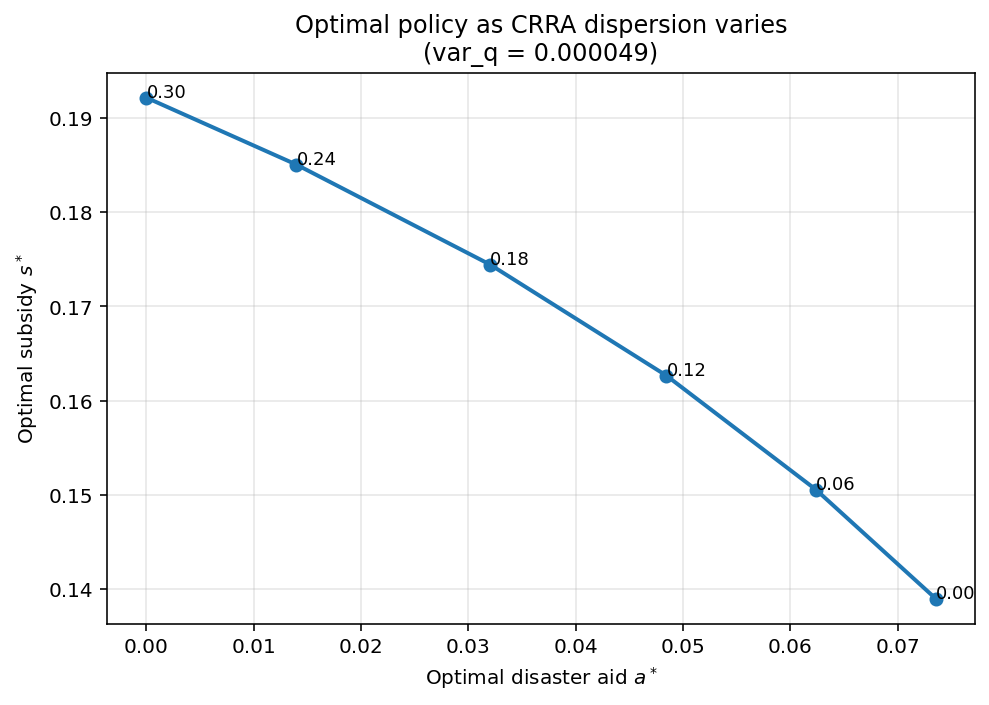
\includegraphics[width=0.7\linewidth]{figures/Dependence_optimalpolicy_vargamma.png}
    \caption{Optimal policy mix with $\sigma_q=0.7\%$. The dots indicate different levels of the variance of risk aversion $\gamma$.}
    \label{fig:optpolicy_gamma}
\end{figure}
\end{document}